%useful packages
\documentclass[12pt]{article}

\usepackage[english]{babel}
\usepackage[margin=1in]{geometry} 
\usepackage{amsmath,amsthm,amssymb,mathtools}
\usepackage{hyperref}
\usepackage{tikz,tkz-euclide,tkz-base}
\usepackage{thmtools}
\usepackage{comment}


\usepackage{listings}
\lstset{language=C++,
                keywordstyle=\color{blue},
                stringstyle=\color{red},
                commentstyle=\color{green},
                basicstyle=\footnotesize,% basic font setting
}

\usetkzobj{all}


\DeclarePairedDelimiter{\ceil}{\lceil}{\rceil}


\DeclareMathOperator{\range}{range}

\newcommand{\N}{\mathbb{N}}
\newcommand{\Z}{\mathbb{Z}}
\newcommand{\R}{\mathbb{R}}
\newcommand{\Q}{\mathbb{Q}}
\newcommand{\C}{\mathbb{C}}
\newcommand{\F}{\mathbb{F}}
\newcommand{\M}{\mathcal{M}}
\newcommand{\seq}{\subseteq}
\newcommand{\norm}[1]{\left\Vert#1\right\Vert}
\newcommand{\angleb}[1]{\left\langle#1\right\rangle}

\renewcommand{\P}{\mathcal{P}}
\renewcommand{\L}{\mathcal{L}}

\DeclareSymbolFont{matha}{OML}{txmi}{m}{it}% txfonts
\DeclareMathSymbol{\vv}{\mathord}{matha}{118}

\AtBeginDocument{\mathcode`v=\vv}


\newenvironment{theorem}[2][Theorem]{\begin{trivlist}
		\item[\hskip \labelsep {\bfseries #1}\hskip \labelsep {\bfseries #2.}]}{\end{trivlist}}

\newenvironment{lemma}[2][Lemma]{\begin{trivlist}
		\item[\hskip \labelsep {\bfseries #1}\hskip \labelsep {\bfseries #2.}]}{\end{trivlist}}

\newenvironment{exercise}[2][Exercise]{\begin{trivlist}
		\item[\hskip \labelsep {\bfseries #1}\hskip \labelsep {\bfseries #2.}]}{\end{trivlist}}

\newenvironment{corollary}[2][Corollary]{\begin{trivlist}
		\item[\hskip \labelsep {\bfseries #1}\hskip \labelsep {\bfseries #2.}]}{\end{trivlist}}

\newenvironment{solution}{\noindent\textit{Solution.}}{\qed}

\hypersetup{linktoc=all, colorlinks=true, linkcolor=black}


\begin{document}
\title{Title}
\author{Author}
\date{9 September 2017}
\maketitle

\section{Introduction}
This document gives a brief overview of a 7-stage 2-issues pipelined RISC processor.

\section{Pipeline Stages}
\subsection{Fetch stage}
The fetch stage is the stage responsible for accessing the instruction memory.
Note that two memories are used: one for instructions, and the other for data.
And since this is a two-issue processor, we fetch two instructions instead of one. 
The fetch buffer consists of:
\begin{enumerate}
	\item \texttt{NOP1:} A one-bit flag to indicate if the first issue is a NOP.
	\item \texttt{IR1:} The instruction word of the first issue.
	\item \texttt{NOP2:} A one-bit flag to indicate if the second issue is a NOP.
	\item \texttt{IR2:} The instruction word of the second issue.
\end{enumerate}
\subsubsection{PC generator }

\begin{figure}
	\centering
	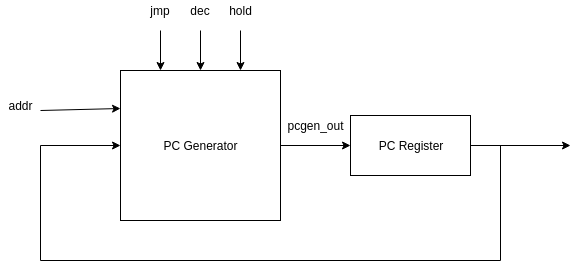
\includegraphics[width=0.7\linewidth]{figures/PCGen.png}
	\caption{A schematic of the PC generator.}
	\label{fig:pcgen}
\end{figure}


The PC generator is a combinational circuit responsible
for updating the PC every clock-cycle. See Figure \ref{fig:pcgen} for a schematic of the component.
There are four cases:
\begin{enumerate}
\item $PC \leftarrow [PC] + 2$. This is the normal case.
\item $PC \leftarrow address$. Needed with jumps and function calls.
\item $PC \leftarrow [PC] - dec$. This is used with incompatible issues.
\item $PC \leftarrow [PC]$. The PC needs to holds its value if the pipe is being stalled.
\end{enumerate}
We define the functionality of the generator with the following priority:
\begin{lstlisting}[escapeinside={(*}{*)}]
	if	(jump)		pcgen_out = addr
	else if	(hold)		pcgen_out = PC
	else if	(dec != 0)	pcgen_out = PC - dec
	else			pcgen_out = PC + 2
\end{lstlisting}

\subsection{Pre-decode stage}
\begin{figure}
	\centering
	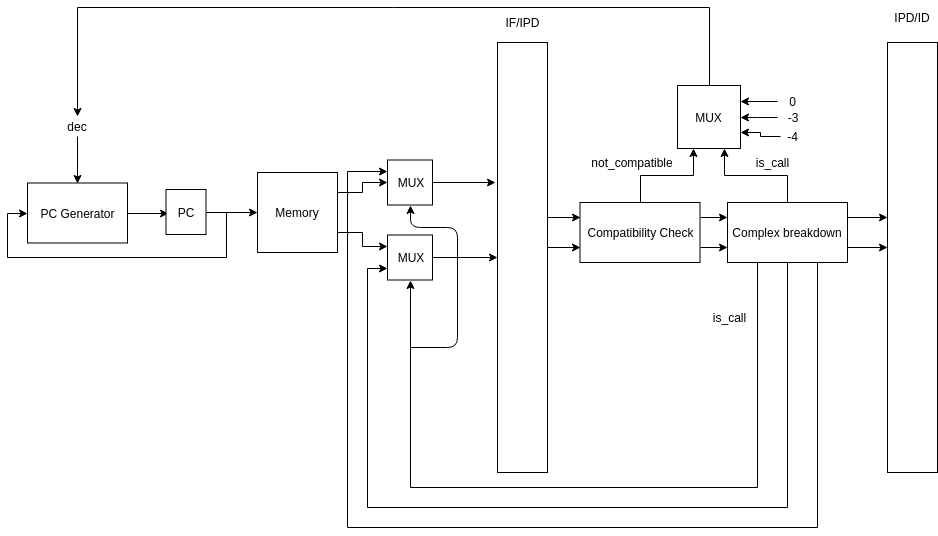
\includegraphics[width=\linewidth]{figures/predecode.png}
	\caption{A schematic of the pre-decode stage.}
	\label{fig:predecode}
\end{figure}

 The Pre-decode stage is responsible for:
 \begin{enumerate}
	\item Checking that two issues are compatible.
	\item Breaking complex instructions into simpler ones.
 \end{enumerate}
 The \texttt{IPD/ID} buffer consists of: 
 \begin{enumerate}
	\item \texttt{NOP1:} A one-bit flag to indicate if the first issue is a NOP.
	\item \texttt{IR1:} The instruction word of the first issue.
	\item \texttt{NOP2:} A one-bit flag to indicate if the second issue is a NOP.
	\item \texttt{IR2:} The instruction word of the second issue.
\end{enumerate}
\subsubsection{Non-compatible Issues}
Any two issues are not compatible if one of the following conditions holds:
\begin{enumerate}
\item One of the issues is a \texttt{push} or \texttt{pop} instruction.
\item One of the issues is a \texttt{call} instruction.
\item The first issue is a branch or change of control operation.
\item The first issue loads a value, and the second uses it.
\item The second issue is \texttt{LDM}.
\item Both of the issues use the memory.
\end{enumerate}
If two issues are not compatible, a signal is sent to the PC generator to decrement by 3, the second issue becomes NOP, and the previous stage is flushed.
The Pre-decode  buffer structure: 

\subsubsection{Complex Instructions}
The following instructions are considered complex:
\begin{enumerate}
\item \emph{PUSH Rdst:} This does two operations: it stores \texttt{Rdst} in \texttt{@SP} and decrements \texttt{SP}. Hence it's broken into:
\begin{lstlisting}
	STD	Rdst, SP
	DEC	SP
\end{lstlisting}
\item \emph{POP Rdst:} Similar to \texttt{PUSH}. It's broken into
\begin{lstlisting}
	INC	SP
	LDD	Rdst, SP
\end{lstlisting}
\item \emph{CALL Rdst:} This one requires special treatment, since it gets broken into 3 instructions, which needs two packets:
\begin{lstlisting}
	STD	PC,	SP
	DEC	SP
	MOV	PC,	Rdst
\end{lstlisting}
In this case, the \texttt{PC} is decremented by 4, and it writes to the \texttt{IF/IPD} buffer the third instruction \texttt{MOV PC, Rdst} instead of reading it from memory.
\end{enumerate}

\subsection{Decode stage}
\begin{figure}
	\centering
	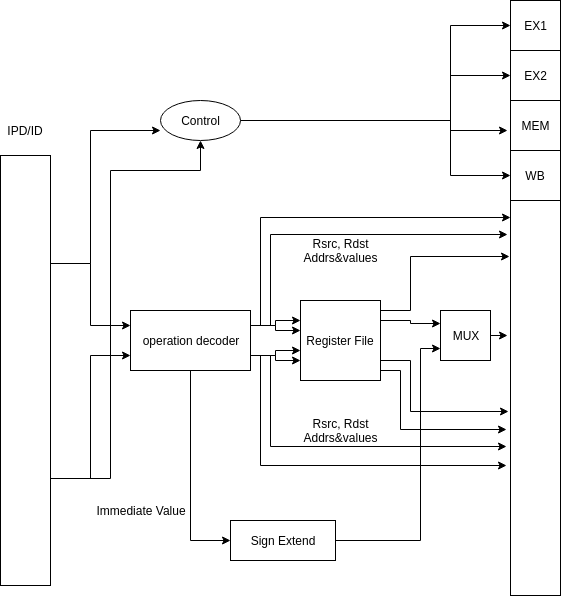
\includegraphics[width=\linewidth]{figures/decode.png}
	\caption{A schematic of the decode stage.}
	\label{fig:decode}
\end{figure}
See Figure \ref{fig:decode} for a schematic of the stage.
The Decode stage is responsible for:
\begin{enumerate}
\item Decoding the relevant registers and reading their values. This is done through the combinational circuit 'operation decoder'. The register file allows the decoder to read four registers at once (two for each issue). It then stores their addresses and values to \texttt{ID/EX1} buffer. 
\item Generates the control values for the next stages, which is done through the 'control' circuit.
\item Sign-extending the immediate value following an \texttt{LDM} instruction, storing it in the buffer's \texttt{Rsrc1} register, and giving it an appropriate \texttt{Rsrc} address.
\end{enumerate}
The \texttt{ID/EX1} buffer consists of:
 \begin{enumerate}
\item \texttt{NOP1 \& NOP2} flags.
\item \texttt{EX1 \& EX2 \& MEM \& WB} Control words.  
\item \texttt{Rsrc1 \& Rdst1} addresses and values.
\item \texttt{Rsrc2 \& Rdst2} addresses and values.
\end{enumerate}
We note that the addresses are 5-bit values. This makes it easier to address the \texttt{PC} and \texttt{SP} registers, and to indicate immediate values (not register).

\subsubsection{Control Unit}
The control unit is responsible for generating the control signals for \texttt{EX1, EX2, MEM} and \texttt{WB} stages. These are:
\begin{enumerate}
\item \texttt{EX1}: The ALU operation \texttt{ALUOp}. Update flag register \texttt{IsFlag}.
\item \texttt{EX2}: The ALU operation \texttt{ALUOp}, a bit indicating branch instruction \texttt{IsBranch}, and a bit indicating whtether to update the flag register \texttt{IsFlag}.
\item \texttt{MEM}: Index of the issue that needs the memory (if any) \texttt{MEMIssueIndex}, and operation \texttt{R/W}.
\item \texttt{WB}: Whether issue 1 or 2 (or both) require write back \texttt{IsWB1}, \texttt{IsWB2}.
\end{enumerate}

\subsection{Execute stage}
This stage is divided into two substages. Dividing the execution into two helps solving RAW dependencies between issues inside the same packet.

\noindent The first execute stage is responsible for executing the ALU operations for the first instruction using the first ALU. 
The \texttt{EX1/EX2} buffer consists of:
\begin{enumerate}
	\item \texttt{NOP1 \& NOP2} flags.
	\item \texttt{EX2 \& MEM \& WB} Control words.  
	\item \texttt{Rsrc1 \& Rdst1} addresses and values.
	\item \texttt{Rsrc2 \& Rdst2} addresses and values.
\end{enumerate}

\noindent The second execute stage is responsible for:
\begin{enumerate}
\item Executing the ALU operations for the second instruction using the second ALU. It benefits from the previous execute stage since it has the ability to have the previous ALU's output as its input through a multiplexer. Which may be considered a kind of forwarding between issues.
\item Executing branch instructions.
\end{enumerate}
The \texttt{EX2/MEM} buffer consists of:
\begin{enumerate}
	\item \texttt{NOP1 \& NOP2} flags.
	\item \texttt{MEM \& WB} Control words.  
	\item \texttt{Rsrc1 \& Rdst1} addresses and values.
	\item \texttt{Rsrc2 \& Rdst2} addresses and values.
\end{enumerate}

\subsection{Memory stage}
It is the stage responsible for accessing the data memory, either to store or load a value. The \texttt{MEM/WB} buffer consists of: 
\begin{enumerate}
	\item \texttt{NOP1 \& NOP2} flags.
	\item \texttt{WB} Control word.  
	\item \texttt{Rsrc1 \& Rdst1} addresses and values.
	\item \texttt{Rsrc2 \& Rdst2} addresses and values.
\end{enumerate}
\subsection{Write back stage}
It is the final stage and the stage responsible for writing back to the register file through the interfacing circuit Register-Write block. This can write to both general registers, and special registers like \texttt{PC} and \texttt{SP}.

\section{Hazards}
\subsection{Data Hazards}
Full forwarding is used between \texttt{EX1}, \texttt{EX2}, \texttt{MEM} and \texttt{WB} stages. Although this solves many of the hazards, it doesn't solve all of them. Stalling is required for these cases:
\begin{enumerate}
\item Between first and fourth packet: Stall 1 cycle in the decode stage if (second issue in fourth packet is ALU instruction or any issue is memory instruction) and depends on any issue in the first packet
\begin{lstlisting}
IF	IPD	ID	EX1	EX2	MEM	WB
	IF	IPD	ID	EX1	EX2	MEM	WB
		IF	IPD	ID	EX1	EX2	MEM	WB
			IF	IPD	ID	ID	EX1	EX2
\end{lstlisting}

\item Between first and third packet: Stall 2 cycles in the decode stage if any issue in third packet is memory instruction, and it has dependency with any issue in the first packet. Or any issue in the first packet is a load instruction, and it has dependency with the first issue in the first packet if it's an ALU instruction.
\begin{lstlisting}
IF	IPD	ID	EX1	EX2	MEM	WB
	IF	IPD	ID	EX1	EX2	MEM	WB
		IF	IPD	ID	ID	ID	EX1	EX2
\end{lstlisting}
\item Between first and second packet: Stall 1 cycle if load-use case happens. Or if the first issue in the second packet depends on the first issue in the first packet, and both are ALU instructions.
\begin{lstlisting}
IF	IPD	ID	EX1	EX2	MEM	WB
	IF	IPD	IPD	ID	EX1	EX2	MEM	WB
\end{lstlisting}
\end{enumerate}
Note that these cases can be easily translated into conditions between stages.

\subsection{Branches \& Control Hazards}
Branches are executed in the \texttt{EX2} stage, and are always predicted to be untaken. If a branch is taken, the EX2 stage does the following:
\begin{enumerate}
\item Disables the load signal on the ALU flag register.
\item Sends the value of the new address to the PC generator and enables the PC generator jmp signal.
\item Flushes previous stages.
\end{enumerate}


\section{Opcodes}
\textbf{IR:}

\begin{tabular}{llll}
	\emph{Two Operand: } & 5 bit opcode & 3 bit reg1 & 3 bit reg2\\
	\emph{One Operand: } & 5 bit opcode & 3 bit reg &\\
	\emph{Branch: } 	& 5 bit opcode & 3 bit reg & \\ 
	\emph{MEM: } & 5 bit opcode & 3 bit reg1 & 3 bit reg2 \\
	\emph{MEM: } & 5 bit opcode & 3 bit reg1 \\
\end{tabular}

\begin{table}[]
	\centering
	\begin{tabular}{ll}
	\hline
	Operation & Opcode \\ \hline
	NOP       & 00 000 \\
	SETC      & 00 001 \\
	CLRC      & 00 010 \\
	NOT       & 00 011 \\
	INC       & 00 100 \\
	DEC       & 00 101 \\
	OUT       & 00 110 \\
	IN        & 00 111 \\
	MOV       & 01 000 \\
	ADD       & 01 001 \\
	SUB       & 01 010 \\
	AND       & 01 011 \\
	OR        & 01 100 \\
	SHL       & 01 101 \\
	SHR       & 01 110 \\
	PUSH      & 11 000 \\
	POP       & 11 001 \\
	LDM       & 11 010 \\
	LDD       & 11 011 \\
	STD       & 11 100 \\
	RESET     & 11 101 \\
	INT       & 11 110 \\
	JZ        & 10 000 \\
	JN        & 10 001 \\
	JC        & 10 010 \\
	JMP       & 10 011 \\
	CALL      & 10 100 \\
	RET       & 10 101 \\
	RETI      & 10 110 \\ \hline
	\end{tabular}
	\end{table}

\end{document}